\chapter{Interactions lumière-matière}
Ce modèle est loin de la réalité mais "correct" en pratique. Il est donc intéressant pour développer une 
certaine intuition du problème.

	\section{Propagation d'onde EM dans un milieu diélectrique}
	\subsection{Approche "particulaire"}
	\begin{wrapfigure}[8]{l}{6cm}
	\vspace{-5mm}
	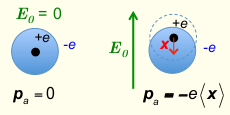
\includegraphics[scale=0.65]{ch2/image1.png}
	\captionof{figure}{ }
	\end{wrapfigure}
	Si la lumière se propage dans un milieu non vide, il y aura des interactions : comment on pourrait décrire 
	ces interactions et d'où elles viennent? Lorsque l'on applique un champ électrique $\vec{E}$ à un système de
	charges, elles ont la possibilité de bouger : le nuage électronique se déforme et il apparaît un moment 
	dipolaire électrique
	\begin{equation}
	\vec{p}_a = -\int e|\psi|^2\vec{r}\ d\vec{r}
	\end{equation}
	où $-e|\psi|^2\ d\vec{r}$ est l'élément de charge à la position $\vec{r}$ donnant lieu à une intégrale 
	non nulle\footnote{Si cette intégrale est nulle lorsque $\vec{E}=\vec{0}$, c'est du au fait que la fonction 
	d'onde est antisymétrique.}. Dans un milieu contenant $N$ atome par unité de volume, la polarisation 
	(macroscopique) est donnée par
	\begin{equation}
	\vec P = N\vec{p_a}
	\end{equation}
	soit la densité atomique multiplié par le moment dipolaire de chaque atome (on suppose que tous les dipôles
	sont orientés dans le même sens).\\
	
	\begin{wrapfigure}[6]{r}{4cm}
	\vspace{-5mm}
	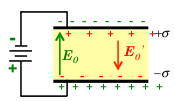
\includegraphics[scale=0.7]{ch2/image2.png}
	\captionof{figure}{ }
	\end{wrapfigure}
	Pour illustrer, penchons-nous sur le cas du condensateur en prenant l'hypothèse d'un milieu linéaire et 
	isotrope (sans quoi la susceptibilité $\chi$ serait un tenseur). Dans ce cas, la polarisation va être
	 proportionnelle à l'amplitude du champ total $E=E_0+E_0'$ où $E_0$ est le champ initial et $E_0'$ le 
	 champ induit.
	 \begin{equation}
	 \left\{\begin{array}{ll}
	 \vec{E_0'} &= -\vec P/\epsilon_0\\
	 \vec E &= \vec E_0-\vec P/\epsilon_0
	 \end{array}\right.\qquad\Rightarrow \vec{P} = \varepsilon_0\chi\vec{E}
	 \end{equation}
	où $\chi$ est la \textbf{susceptibilité électrique}.
	
	Calculons la divergence de ce champ électrique total
	\begin{equation}
	\div \vec{E} = \div(\vec{E_0}-\vec{P}/\epsilon_0)\quad \Leftrightarrow\quad \div(\vec{E}+\vec{P}/\epsilon_0) 
	= \div(\vec{E_0})
	\end{equation}
	Dans le vide $\div(\vec{E_0}) = \rho_{libre}/\epsilon_0$. Pour tenir compte de l'apparition des dipôles, 
	on introduit un \textbf{champ de déplacement} $D$ de sorte à pouvoir écrire une formule de divergence 
	"classique". Par définition
	\begin{equation}
	\vec{D} = \varepsilon_0\vec{E}+ \vec{P} = \varepsilon_0(1+\chi)\vec{E} = \varepsilon\vec{E}
	\end{equation}
	où $\varepsilon_r = \varepsilon/\varepsilon_0 = (1+\chi)$.	On peut alors écrire
	\begin{equation}
	\div\vec{D} = \rho_{libre}
	\end{equation}
	En toute généralité, cette susceptibilité $\chi$ sera complexe : absorption, gain, \dots en découleront.
	
	
	En toute généralité, le champ électrique peut varier dans le temps. On défini alors la \textbf{densité de courant} (densité d'électron * charge * variation de la position de cette charge) :
	$\vec{J}$
	\begin{equation}
	J_{liee} = -Ne\dfrac{d}{dt}\langle x \rangle \quad\Leftrightarrow\quad J_{liee} = N\dfrac{d}{dt}\vec{p_a} =
	\dfrac{d}{dt}\vec{P}
	\end{equation}
	Il y aura toujours un dipôle accompagné d'un moment dipolaire atomique mais cette fois-ci dépendant du temps.\\
	
	
Partons maintenant des équations de Maxwell et des équations constitutives. Considérons 
	un milieu diélectrique ($\rho_{libre}=0$) et non magnétique ($\vec{B}=\mu_0\vec{H}$)
	\begin{equation}
	\left\{\begin{array}{ll}
	\rot\vec{E} &\DS= -\frac{\partial}{\partial t}\vec{B}\\
	\rot\vec{B} &\DS=\mu_0\dfrac{\partial}{\partial t}\vec{D}\\
	\div\vec{D}&=\DS 0\\
	\div\vec{B}&=\DS 0
	\end{array}\right.\qquad\qquad\text{ et }\qquad\qquad\left\{\begin{array}{ll}
	\vec{D} &=\DS \varepsilon\vec{E} = \varepsilon_0\vec{E}+\vec{P}\\
	\vec{B}&=\DS \mu_0\vec{H}
	\end{array}\right.
	\end{equation}
	En calculant le rotationnel du rotationnel du champ électrique\footnote{$\rot\rot = \div\div - \Delta$}, 
	on trouve l'équation d'onde
	\begin{equation}
	\Delta\vec{E}-\frac{1}{c^2}\dfrac{\partial^2}{\partial^2}\vec{E}=\mu_0\dfrac{\partial^2}{\partial t^2}\vec{P}
	\end{equation}
	où $c = 1/\sqrt{\epsilon_0\mu_0}$ est la vitesse de la lumière dans le vide. \\
	
	Trois cas sont particulièrement intéressants
	\begin{enumerate}
	\item	Dans le vide : $\vec{P}=\vec{0}$ et on retrouve la solution harmonique, décrite par des ondes planes
	\begin{equation}
	\vec{E} = \frac{1}{2}(\mathcal{E}\exp(i(\vec{k}.\vec{r}-\omega t))\vec{e} + c.c.)
	\end{equation}
	où $\vec{e}$ est le vecteur de polarisation. Pour que ce soit bien solutions des équations de Maxwell, il 
	faut que $\vec{k}.\vec{e} = 0$ (polarisation transverse) et $|\vec{k}| = \omega/c=2\pi/\lambda_0$.\\
	\item Dans un diélectrique, la polarisation varie dans le temps : effets de réfractions, de perte et de gain
	\item \textbf{Indice de réfraction complexe} $\mathcal{N}$.\\
	Soit la solution harmonique et $\vec{k}=\mathcal{K}.\vec{1_z}$
	Jusqu'ici, nous avons toujours considéré que l'indice de réfraction n'était du qu'à des effets de phase.

	Adoptons des notations en phaseurs
	\begin{equation}
	\vec{E} =\frac{1}{2}(\mathcal{E}\exp(i(\mathcal{K}z-\omega t))\vec{e} + c.c.)= \frac{1}{2}(\hat{\vec{E}}+c.c.),\qquad\qquad\vec{P} = \frac{1}{2}(\hat{\vec{p}}+c.c.)
	\end{equation}
	où nous avons cette fois-ci autorisé $\mathcal{K}$ à être complexe. En faisant de même pour $\hat{\vec{P}}$ 
	(par identification) :
	\begin{equation}
	\hat{\vec{P}} = \varepsilon_0\chi\hat{\vec{E}} = \varepsilon_0(\chi'+i\chi'')\hat{\vec{E}}
	\end{equation}
	Après substitution de ces équations dans l'équation de propagation (la dérivée en $z$ fait apparaître un 
	$\mathcal{K}^2$.
	\begin{equation}
	\mathcal{K}^2 = \dfrac{\omega^2}{c^2}(1+\chi'+i\chi'')
	\end{equation}
	où l'on note $\mathcal{K}=k+i\alpha_E$ où $\alpha_E$ est le coefficient d'atténuation du champ électrique. Si 
	l'on substitue cette nouvelle expression de $\mathcal{K}$ dans l'expression de $\vec{E}$, on fait apparaître 
	une exponentielle négative
	\begin{equation}
	\vec{E}=\mathcal{E}\exp(-\alpha_Ez)\cos(kz-\omega t)
	\end{equation}
	On définit le coefficient d'absorption en énergie $\alpha=2\alpha_E$. Si $\alpha>0$ il s'agit d'un milieu à
	 pertes (à gain, inversement).\\
	 
	Venons-en à ce qui nous intéresse ici : l'\textbf{indice de réfraction complexe} défini
	\begin{equation}
	\mathcal{N} = \eta +i\kappa
	\end{equation}
	tel que $\mathcal{K}=\dfrac{\omega}{c}\mathcal{N}$. Le champ électrique établi ci-dessus devient alors
	\begin{equation}
	\vec{E} =\vec{\mathcal{E}}\exp\left[-\frac{\omega}{c}\kappa z\right]\cos\left(\frac{\omega}{c}\eta z-\omega t\right)
	\end{equation}
	L’absorption vaut alors $\alpha = 2\frac{\omega}{c}\kappa$ et la vitesse de phase $v_\phi = \frac{\omega}
	{c}=\frac{c}{\eta} \to \lambda=\frac{\lambda_0}{\eta}$
	En identifiant la partie réelle et imaginaire :
	\begin{equation}
	\left\{\begin{array}{ll}
	\eta^2-\kappa^2 &= 1+\chi'\\
	\eta\kappa &= \chi''/2
	\end{array}\right.
	\end{equation}
	Souvent on peut entendre que la partie réelle correspond à des effets de phase ($\vec{k}$) alors que la partie 
	imaginaire correspond à des pertes/gain : ce n'est pas exact, les deux sont "mélangés". Cependant, si 
	$\kappa\ll 1$
	\begin{equation}
	\left\{\begin{array}{ll}
	\eta &\approx \sqrt{1+\chi'}\\
	\kappa &\approx \chi''/(2\sqrt{1+\chi'})
	\end{array}\right.
	\end{equation}
	On remarque que $\eta,\kappa$ dépendent de $\omega$. On nomme alors \textbf{relation de dispersion} l'équation $\eta = f(\omega)$.
	\end{enumerate}
	
	\subsection{Modèle de l'oscillateur harmonique}
	Le souci est que nous ne connaissons pas les expression de $\eta, \kappa, \chi'$ et $\chi''$, tous fonction 
	de $\omega$. On va utilisé un modèle qualitativement correct (mais assez loin de la réalité) pour les obtenir 
	dans un milieu diélectrique isotrope (gaz,ions dans un solide,\dots)\\
	
	Considérons \textit{un} électron élastiquement (constante de rappel $k$) lié à un noyau infiniment lourd sur
	lequel on applique $E(t)$. On introduit un terme de relaxation (damping) $m\gamma\dot{x}(t)$ si on veut une
	description assez fidèle, le nuage électronique ne peut osciller infiniment \footnote{Une densité de charge liée
	bougeant agit comme une antenne : émission d'onde EM.}. Il faut donc perdre de l'énergie, ce qui est le rôle de
	ce terme. Nous obtenons alors
	\begin{equation}
	\ddot{x}(t) + \omega_a^2(t)+\gamma\dot{x}(t) = -\frac{eE(t)}{m}
	\end{equation}
	où $\omega_a = \sqrt{k/m}$, $\frac{1}{\gamma}$ est le temps caractéristique de relaxation pour la polarisation 
	$\vec{P}$ et le membre de droite comporte le terme d'oscillation forcée. En utilisant les deux phaseurs
	\begin{equation}
	E(t) = \frac{\mathcal{E}\exp(-i\omega t) + c.c.}{2},\qquad\qquad
	x(t) = \frac{X\exp(-i\omega t) + c.c.}{2}
	\end{equation}
	On trouve
	\begin{equation}
	(\omega_a^2-\omega^2-i\gamma\omega)X\exp(-i\omega t)+c.c. = \frac{e\mathcal{E}}{m}\exp(-i\omega t)+c.c.
	\end{equation}
	Sachant que $\vec{P}=-eN\vec{x}(t)=\frac{\hat{\vec{P}}+c.c.}{2}$ où $\hat{\vec{P}}=\varepsilon_0\chi\hat{
	\vec{E}}$, on trouve
	\begin{equation}
	\chi(\omega) = \dfrac{Ne^2}{\varepsilon_0m}\dfrac{1}{\omega_a^2-\omega^2-i\gamma\omega}
	\end{equation}
	Comme $\chi$ est complexe, il peut y avoir un déphasage entre l'excitation et la position du système 
	masse-ressort
	Les parties réelles et imaginaires valent alors
	\begin{equation}
	\chi'(\omega) = \dfrac{Ne^2}{\varepsilon_0m}\dfrac{\omega_a^2-\omega^2}{(\omega_a^2-\omega^2)^2+\gamma^2
	\omega^2},\qquad\qquad\chi''(\omega) = \dfrac{Ne^2}{\varepsilon_0m}\dfrac{\gamma\omega}{(\omega_a^2-\omega^2)^2+\gamma^2
	\omega^2}
	\end{equation}
	Jusqu'ici, nous travaillons sans approximations mais ces résultats ne sont pas évident à interpréter. Pour 
	se faire, nous allons faire l'hypothèse que l'amortissement est lent. Dès lors, $\vec{E}$ fait un grand 
	nombre d'oscillation avant une atténuation totale du système masse-ressort
	\begin{equation}
	\omega_a^2-\omega^2 = 2\omega_a(\omega_a-\omega)
	\end{equation}
	Avec cette hypothèse, $\chi''$ devient directement proportionnel à $\alpha$ et on le montrera. Il s'agit 
	d'une \textit{lorentzienne}
	\begin{equation}
	\chi''(\omega) = \dfrac{Ne^2}{\varepsilon_0m\gamma\omega_a}\dfrac{1}{1+\frac{(\omega_a-\omega)^2}{(\gamma
	/2)^2}} > 0
	\end{equation}
	
	\begin{wrapfigure}[6]{l}{6.5cm}
	\vspace{-5mm}
	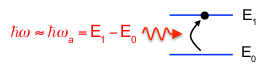
\includegraphics[scale=0.7]{ch2/image3.png}
	\captionof{figure}{ }
	\end{wrapfigure}
	Cette fonction est positive $\forall\omega$, ce qui implique que $\alpha$ sera toujours positif ce qui 
	correspond à de l'absorption : passage d'un niveau fondamental vers un état excité.\\
	Pour $\chi'(\omega)$, on trouve
	\begin{equation}
	\chi'(\omega) = \dfrac{Ne^2}{\varepsilon_0m\gamma\omega_a}\dfrac{(\omega_a-\omega)/(\gamma/2)}
	{1+\frac{(\omega_a-\omega)^2}{(\gamma	/2)^2}}
	\end{equation}
	Ceci met en évidence une variation de l'indice de réfraction : c'est une relation de dispersion. 
	
	\newpage
	Traçons ces deux courbes. Ci-dessous, en rouge, nous avons une absorptions. En vert, une variation de
	l'indice de réfraction : nous verrons que s'il y a un effet d’absorption, il y a forcément un effet 
	de réfraction $\eta$ alors que $\kappa \propto \chi''(\omega)$
	\begin{center}
	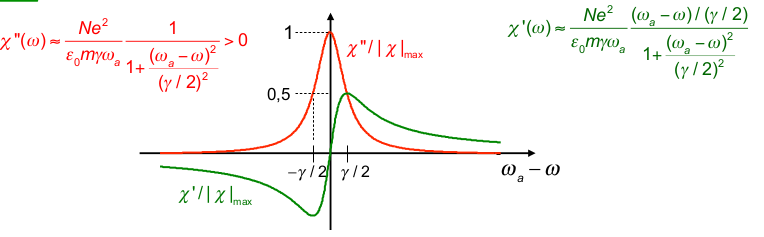
\includegraphics[scale=0.5]{ch2/image4.png}
	\captionof{figure}{ }
	\end{center}	
	Si l'on excite le système en balayant sur les fréquences, nous observerons des pics d'absorption 
	($\kappa$) et une modification de $\eta$. Le verre se situe entre deux pics : il est transparent 
	car il n'y a pas d’absorption par contre on observe tout de même une variation de l'indice de 
	réfraction permettant de distinguer les différentes couleurs.
	\begin{center}
	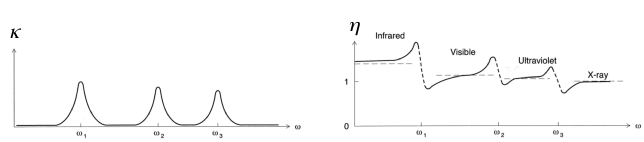
\includegraphics[scale=0.7]{ch2/image5.png}
	\captionof{figure}{ }
	\end{center}	
	
	\newpage
	\section{Particule de lumière}
	\subsection{Équations de Maxwell : onde électromagnétique}
	Jusqu'ici nous avons utilisé une approche électromagnétique : passons cette fois-ci à une approche
	corpusculaire. Intéressons-nous à l'énergie (ce qui est quantifié). On s'intéresse à l'intensité ($W
	/m^2$) qui est liée au vecteur de Poyting $\vec{\mathcal{S}}=\vec{E}\times\vec{H}$ et on en prend la
	moyenne\footnote{Un flux d'énergie oscillant n'a pas de sens.} 
	\begin{equation}
	I = \langle|\vec{\mathcal{S}}|\rangle = \langle|\vec{E}\times\vec{H}\rangle = \frac{1}{2}\varepsilon_0
	\eta\mathcal{E}^2
\end{equation}		
	La solution harmonique des équations de Maxwell étant
	\begin{equation}
	\vec{E} = \mathcal{E}\cos(kz-\omega t)\vec{e}
	\end{equation}
	Nous remarquons qu'il n'y a aucune condition sur l'amplitude $\mathcal{E}$ qui peut varier de façon 
	continue : de même pour l'intensité. Toutes les énergies seraient alors possibles ce qui est faux 
	expérimentalement (effet photoélectrique notamment). 
	
	\subsection{Lumière : un ensemble de photons}
	Planck par l'étude du corps noir et Einstein avec l'effet photoélectrique ont proposés une quantification
	du champ électromagnétique : les quanta de lumières ont une énergie $\Delta E = \hbar\omega$.
	
	\subsection{Description simplifiée de la quantification des champs EM}
	\begin{wrapfigure}[10]{l}{7.5cm}
	\vspace{-5mm}
	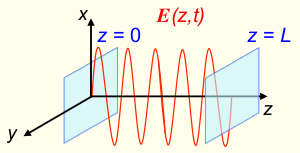
\includegraphics[scale=0.7]{ch2/image6.png}
	\captionof{figure}{ }
	\end{wrapfigure}
	Supposons une cavité vide (pas de radiation, charge, milieu diélectrique), unidimensionnelle selon $z$ 
	formée de murs parfaitement conducteurs (un miroir parfait, rien ne sort de la cavité) en $z=0,L$ où passe
	 un champ $\vec{E}$ polarisé selon $x$. Nous allons toujours appliquer les équations de Maxwell, mais avec 
	 ces conditions de cavité
	\begin{equation}
	\dfrac{\partial^2}{\partial z^2}E_x(z,t) -\frac{1}{c^2}\dfrac{\partial^2}{\partial t^2}E_x(z,t)=0
	\end{equation}
	avec comme CL $E_x=0$ en $z=0,L$. La solution n'est rien d'autre que l'harmonique
	\begin{equation}
	E_x(z,t) = f_0\sin(kz)q(t),\qquad k=\frac{m\pi}{L};\quad m=1,2,\dots
	\end{equation}
	où $E_x$ dépend de $z$ et $t$, $f_0$ est l'amplitude multipliée par la variation spatiale et par une 
	fonction non définie. C'est exactement ce que nous avions obtenu (et heureusement, nous décrivons la 
	même chose). On en tire facilement le champ magnétique
	\begin{equation}
	B_y(z,t) = \frac{\mu_0\varepsilon_0}{k}f_0\cos(kz)\dot{q}
	\end{equation}
	où $\dot{q} =\frac{dq}{dt}$. Ces deux équations, pour $m$ fixé, forment un \textbf{mode de cavité} pour 
	le champ électromagnétique de fréquence angulaire $\omega = m\pi c/L$.\\
	
	Intéressons-nous à l'énergie totale d'un mode : il s'agit de la densité d'énergie du champ magnétique 
	et du champ électrique. 
	\begin{equation}
	H = \int\left[\frac{1}{2}\varepsilon_0E_x^2+\frac{1}{2\mu_0}B_y^2\right]\ dV
	\end{equation}
	Sachant que $V$ est le volume effectif de la cavité, on trouve
	\begin{equation}
	H = \frac{1}{4}f_0^2\varepsilon_0V\left[\dfrac{\varepsilon_0\mu_0}{k^2}\dot{q}^2\right]
	\end{equation}
	Pour simplifier, on considère la constante de normalisation $\DS f_0=\left(\dfrac{2\omega^2}{
	\varepsilon_0V}\right)^2$ :
	\begin{equation}
	H = \frac{1}{2}(p^2+\omega^2q^2)
	\end{equation}
	Ce qui n'est rien d'autre que l'Hamiltonien de l'oscillateur harmonique où $q$ est la position de la 
	masse et où la force de rappel est $F=-\omega^2 q$ (et $p=\dot{q}$). Par analogie, un mode de champ 
	électromagnétique est équivalent à un oscillateur harmonique qui aurait une masse unitaire et où les 
	champs $\vec{E}$ et $\vec{B}$ jouent le même rôle que la position et le moment. L'idée venant 
	naturellement est alors d'essayer de quantifier cette O.H. en utilisant le principe de correspondance 
	$p\to\hat{p}, q\to\hat{q}$ tel que $\hat{p}=-i\hbar \nabla$. \\
	
	Passons donc en mécanique quantique sans se soucier que $H$ est l'énergie d'un cas classique. L'équation 
	de Schrödinger indépendante du temps s'écrit
	\begin{equation}
	\left(\dfrac{\hbar^2}{2}\dfrac{d}{dq^2}+\dfrac{\omega^2}{2}q^2\right)\phi(q) = E\phi(q)
	\end{equation}
	On trouve comme énergie quantifiée
	\begin{equation}
	E_n = \left(n_p+\dfrac{1}{2}\right)\hbar\omega
	\end{equation}
	où on va interpréter $n_p$ comme le nombre de photons contenus dans la cavité considérée. On nomme 
	$E_0$ les \textit{fluctuations du vide} qui peuvent être utile mais pas ici : comme nous allons 
	sommer une infinité de mode, on obtiendrait une énergie infinie. On n'en tiendra donc pas compte.\\
	
	Nous n'avions pas définit $q(t)$ : il s'agit d'une fonction évoluant au cours du temps : celle-ci donnera 
	l'amplitude du champ. L'énergie contenue dans le champ est ainsi proportionnelle au carré de l'amplitude 
	de ce champ ce qui n'est rien d'autre que le cas classique où chaque oscillateur est défini par $\omega, 
	\vec{k}$.
	\begin{equation}
	\langle q\rangle = \bra{\phi}q\ket{\phi} = 0,\qquad\qquad\qquad \langle q^2\rangle\propto E_n
	\end{equation}
	
	\subsection{Flux de photon $\mathcal{J}$ et densité $n_p$}
		\begin{wrapfigure}[6]{l}{7.5cm}
	\vspace{-5mm}
	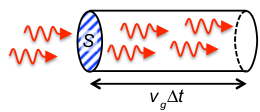
\includegraphics[scale=0.7]{ch2/image7.png}
	\captionof{figure}{ }
	\end{wrapfigure}
	Nous allons suivre la démarche de Planck, à savoir tenter de quantifier le corps noir. Supposons que les 
	photons soient monochromatiques et qu'ils se déplacent à la vitesse de groupe
	\begin{equation}
	v_g = \frac{c}{n_g} = \left(\dfrac{\partial k}{\partial\omega}\right)^{-1}
	\end{equation}
	Il est dès lors utile de s'intéresser au flux du photon car l'intensité peut facilement s'en déduire : 
	l'intensité est donnée par le produit de l'énergie d'un photon par le flux photonique. La valeur moyenne
	du vecteur de Poynting donne l'intensité\footnote{Pq $\mathcal{J}\hbar\omega$ ?}
	\begin{equation}
	\langle |\vec{S}|\rangle = \mathcal{J}\hbar\omega = \frac{1}{2}\varepsilon_0c\eta\mathcal{E}^2 = I\qquad
	\Leftrightarrow\qquad \mathcal{J} = \dfrac{\eta\varepsilon_0c}{2\hbar\omega}\mathcal{E}^2
	\end{equation}
	où $\mathcal{J}$ est le \textbf{flux de photon} [$m^{-2}.s^{-1}$]. On a donc un lien direct entre le flux 
	de photon et le module carré de l'amplitude du champ. A l'aide du schéma ci-dessus, nous pouvons montrer 
	que la \textbf{densité de photon} [$m^{-3}$]vaut 
	\begin{equation}
	\mathcal{J}S\Delta t = n_pSv_G\Delta t\qquad\Leftrightarrow\qquad n_p = \dfrac{\mathcal{J}}{v_g}=
	\dfrac{\eta n_g\varepsilon_0}{2\hbar\omega}\mathcal{E}^2
	\end{equation}
	ce qui n'est \textbf{pas} $n_p$ (nombre de photons).
	
	\section{Cavité radiative}
	Le but est d'obtenir la densité d'énergie par unité de fréquence d'un corps noir. Ce que l'on va faire pour 
	y parvenir, c'est faire un tout petit trou en supposant que l'équilibre thermique n'est pas perturbé, et 
	observer ce qui sort. Planck a ainsi trouvé que la probabilité de trouver un mode à une certaine énergie 
	donnée est donné par la loi de Boltzmann. \\
	La probabilité $p_{np}$ qu'un mode (oscillateur) soit dans l'état $n_p$ est donné par
	\begin{equation}
	p_{n_p} = \dfrac{\exp(-E_{n_p}/k_BT)}{\sum_{n_p=0}^\infty \exp(-E_{n_p}/k_BT)}
	\end{equation}
	où la division par la série permet la normalisation et où $E_{n_p} = (n_p+1/2)\hbar\omega$. Après 
	substitution
	\begin{equation}
	p_{n_p} = \dfrac{\exp(-n_p\hbar\omega/k_BT)}{\sum_{n_p=0}^\infty \exp(-n_p\hbar\omega/k_BT)}
	\end{equation}
	Le nombre moyen de photon est donné par l'espérance mathématique. En adoptant la notation
	\begin{equation}
	\langle n_p\rangle = \sum_{n_p=0}^\infty n_pp_{n_p},\qquad x=\dfrac{\hbar\omega}{k_BT}
	\end{equation}
	On trouve
	\begin{equation}
	\langle n_p\rangle = \dfrac{\sum_{n_p=0}^\infty n_p\exp(-n_p\hbar\omega/k_BT)}{\sum_{n_p=0}^\infty \exp(-n_p\hbar\omega/k_BT)}
	\end{equation}
	Le résultat (numérique et graphique) après résolution des séries est donné ci-dessous.\newpage
	\begin{center}
	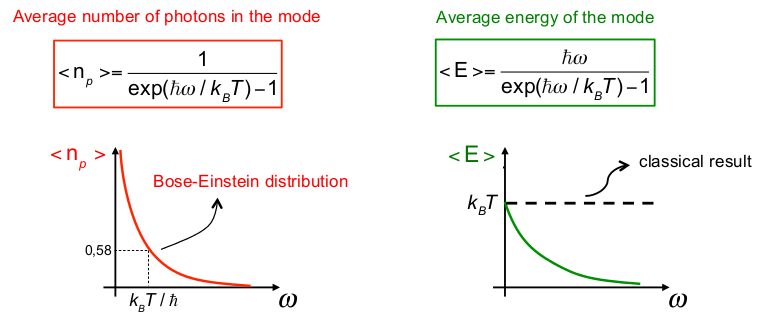
\includegraphics[scale=0.55]{ch2/image8.png}
	\captionof{figure}{ }
	\end{center}
	Le nombre moyen de photons dans un mode est donné par la distribution de Bose-Einstein : sa multiplication 
	par $\hbar\omega$ donne l'énergie moyenne du mode. Il s'agit d'une fonction décroissante tendant vers 
	$k_BT$ lorsque $\omega\to0$.\\
	
	Si l'on effectue le calcul, à température ambiante, il y a à peu près $e^{-100}$ photons visible : ceci 
	est cohérent avec le fait que la lumière ne rayonne pas. Dans un cadre classique, Rayleigh-Jeans avaient 
	obtenu (variation continue d'énergie)
	\begin{equation}
	\langle E\rangle = \dfrac{\int_0^\infty Ee^{-E/k_BT}\ dE}{\int_0^\infty e^{-E/k_BT}\ dE} = k_BT
	\end{equation}
	Ceci est vrai à faible fréquences, mais totalement faux à hautes fréquences.
	
	\subsection{Spectre de la cavité radiative}
	Connaître l'énergie dans un mode n'est que peu intéressant si l'on ne sait pas combien il y a de mode
	par unité de fréquence. On va émettre l'hypothèse que le spectre de la radiation du corps noir est 
	proportionnel à la \textbf{densité spectrale d'énergie} $u(\omega)$ dans la cavité. On va utiliser
	\begin{equation}
	u(\omega)\ d\omega
	\end{equation}
	Il s'agit de la multiplication entre l'énergie moyenne dans un mode par la densité spectrale\footnote{"Combien 
	j'ai de mode par unité de volume par fréquence $\omega$"} en 	énergie, soit le nombre de mode par unité de
	volume dans un intervalle $[\omega,\omega+d\omega]$. Dès lors
	\begin{equation}
	u(\omega)d\omega = \langle E\rangle \rho(\omega)d\omega
	\end{equation}
	\begin{wrapfigure}[6]{r}{4.5cm}
	\vspace{-5mm}
	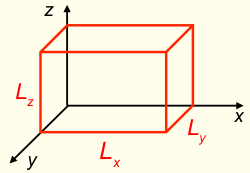
\includegraphics[scale=0.5]{ch2/image9.png}
	\captionof{figure}{ }
	\end{wrapfigure}
	où $\rho(\omega)$ est la densité spectrales des mode dans le champ EM. Intéressons-nous aux nombres de 
	mode par unité de fréquence par unité de volume $\rho(\omega)$ d'une cavité rectangulaire de volume 
	$V=L_1L_2L_3$ (on va montrer que c'est indépendant de la géométrie) composée de murs parfaitement 
	conducteurs et à l'équilibre thermique à la température $T$.
	\newpage
	
	Le slide 19 donne la résolution (par séparation de variable) de ce problèmes aux limites. Si l'on fixe 
	$l,m$ et $n$ le vecteur d'onde est fixé : il y aura deux solutions possibles correspondant à deux 
	polarisations orthogonales. 
	\begin{equation}
	k_x = \frac{l\pi}{L_x},\qquad k_y = \frac{m\pi}{L_y}, \qquad k_z = \frac{n\pi}{L_z}
	\end{equation}
	où $l,m,n=0,1,2,\dots$. Nous pouvons maintenant calculer le nombre de mode présent dans l'intervalle 
	de fréquences $[\omega,\omega+d\omega]$ : ce calcul est plus simple dans l'espace réciproque car une 
	cellule de cette espace à les dimensions $\pi/L_x, \pi/L_y, \pi/L_z$. En notant ce nombre de mode $N_k$, 
	on trouve
	\begin{equation}
	N_k = 2\dfrac{1}{8}\dfrac{4\pi k^2\ dk}{8\frac{\pi}{L_x}\frac{\pi}{L_y}\frac{\pi}{L_z}} = \dfrac{k^2\ dk}
	{\pi^2}V
	\end{equation}
	où nous avons deux états de polarisation, le facteur $1/8$ correspond au huitième de sphère et où l'on a 
	divisé le volume de la calotte sphérique par le volume d'une cellule élémentaire. Sachant que $k^2 =
	\omega^2/c^2 \rightarrow k\ dk = \omega d\omega/c^2$
	\begin{equation}
	\frac{N_\omega}{V} = \rho(\omega)d\omega = \frac{\omega}{c}\frac{\omega d\omega}{\pi^2 c^2}
	\end{equation}
	où nous avons divisé par le volume, voulant une densité. Après intégration, on trouve la densité spectrale 
	de mode
	\begin{equation}
	\rho(\omega) = \dfrac{\omega^2}{\pi^2c^3}
	\end{equation}
	En multipliant par l'énergie moyenne (espérance mathématique), on trouve la \textbf{loi de radiation de 
	Planck}
	\begin{equation}
	u(\omega) = \dfrac{\hbar\omega^3}{\pi^2c^3}\dfrac{1}{e^{\hbar\omega/k_BT}-1}
	\end{equation}
	
	\begin{wrapfigure}[10]{r}{6.5cm}
	\vspace{-5mm}
	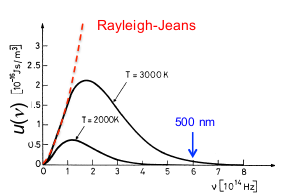
\includegraphics[scale=0.65]{ch2/image10.png}
	\captionof{figure}{ }
	\end{wrapfigure}
	
	Cette expression est en excellent accord avec l'expérience, impliquant une quantification du champ EM. 
	Cette loi n'est strictement valable que pour une cavité fermée en équilibre thermique. Cependant, elle 
	décrit bien les radiations de sources thermiques non nécessairement à l'équilibre thermique, comme le 
	soleil. Si la cavité n'est pas vide (diélectrique) il suffit de remplacer $c$ par $c/\eta$. La 
	généralisation est immédiate
	\begin{equation}
	u(\omega) = \dfrac{\hbar\omega^3\eta^3}{\pi^2c^3}\dfrac{1}{e^{\hbar\omega/k_BT}-1}
	\end{equation}
	Il est possible d'obtenir une telle courbe pour le spectre du soleil. Le seul paramètre libre étant la 
	température, il a été possible de mesurer la température du soleil sans devoir y tremper son doigt. Si 
	l'on regarde la courbe de radiation du corps noir à $T=2.726\ K$ on se rend compte que la courbe 
	ne peut pas plus coller les prédictions expérimentales.
	
	
	
	\newpage
	\section{Interactions dans un milieu à deux niveaux atomiques}
	\subsection{Coefficients d'Einstein}
	Nous allons maintenant considérer le point de vue d'A. Einstein et ses coefficients. Soit 
	un système atomique avec seulement deux niveaux d'énergies $E_1$ et $E_2$ et soit $N_1,N_2$ 
	le nombre d'atome par unité de volume dans chacun de ces niveaux. \\
	
	Il existe plusieurs interactions possibles entre ce système et un champ électromagnétique : 
	nous allons commencer par supposer que tout photon que l'on trouve dans ce système possède 
	une énergie proche de l'écart énergétique entre les deux niveaux : $\hbar\omega_a=E_2-E_1$ où 
	$\omega_a$ est la fréquence de Bohr de la transition. On suppose également que le champ EM 
	a une densité spectrale de radiation $\omega_a$ : $u(\omega_a)$. \\
	
	Notons que $u(\omega_a)$ ne vaut pas forcément celle que nous venons d'obtenir pour le corps
	noir. Pour un laser, nous aurions
	\begin{equation}
	u(\omega_a) = \delta(\omega-\omega_a)\hbar\omega n_p
	\end{equation}
	où $n_p$ est la densité de photon. 	Trois interactions sont possibles 
	\begin{center}
	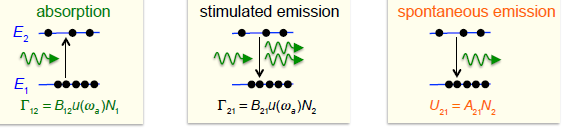
\includegraphics[scale=0.85]{ch2/image11.png}
	\captionof{figure}{ }
	\end{center}
	où $\Gamma_{12} (\Gamma_{21})$ est le taux d'absorption (d'émission stimulée) par unité de 
	volume ($s^{-1}.m^{-3}$), $U_{21}$ est le taux d'émission spontanée par unité de volume et 
	$A_{ij},B_{ij}$ sont les coefficients d'Einstein.\\
	
	On peut alors se demander que vaut $\Gamma_{21}$ pour un photon/mode à $\omega_a$. La seule
	inconnue est $u(\omega_a)$ qui est une énergie par unité de fréquence par unité de volume
	\begin{equation}
	u(\omega_a) = 1*\hbar\omega_a*\left(\dfrac{\omega_a^2}{\hbar^22c^3}*\eta^3\right)
	\end{equation}
	où 1 est le nombre de photon que l'on multiplie par l'énergie et la densité spectrale de mode.\\
	
	Intéressons-nous au cas particulier d'\textit{atomes à l'équilibre thermique dans une cavité 
	à la température $T$.} A l'équilibre, le taux de création doit correspondre au taux d'annihilation
	\begin{equation}
	{B_{12}}u({\omega _a}){N_1} = {B_{21}}u({\omega _a}){N_2} + {A_{21}}{N_2}
	\end{equation}
	On peut en déduire la densité spectrale d'énergie du champ qui permet d'être à cet équilibre
	\begin{equation}
	u({\omega _a}) = \frac{{{A_{21}}}}{{\frac{{{N_1}}}{{{N_2}}}{B_{12}} - {B_{21}}}}
	\end{equation}
	Comme nous sommes en situation d'équilibre, le rapport de $N_1$ et $N_2$ est donné par la 
	statistique de Boltzmann
	\begin{equation}
	\frac{{{N_1}}}{{{N_2}}} = \exp [({E_2} - {E_1})/{k_B}T] = \exp (\hbar {\omega _a}/{k_B}T)
	\end{equation}
	Plank nous donne une autre expression de $u(\omega_a)$ :
	\begin{equation}
	u({\omega _a}) = \frac{{{A_{21}}/{B_{21}}}}{{{B_{12}}/{B_{21}}\exp (\hbar {\omega _a}/{k_B}T) - 1}} = \frac{{\hbar {\omega _a}^3{\eta ^3}}}{{{\pi ^2}{c^3}}}\frac{1}{{\exp (\hbar {\omega _a}/{k_B}T) - 1}}
	\end{equation}
	Ces deux expressions de $u(\omega_a)$ décrivent une cavité fermé à l'équilibre : il s'agit de 
	corps noirs, nous pouvons égaler les deux expressions. On en tire que 
	\begin{equation}
	B_{12} = B_{21},\qquad\qquad \frac{{{A_{21}}}}{{{B_{21}}}} = \frac{{\hbar {\omega _a}^3{\eta ^3}}}
	{{{\pi ^2}{c^3}}}
	\end{equation}
	Dès lors
	\begin{equation}
	\Rightarrow \;\;{U_{21}} = {B_{21}}\rho ({\omega _a})\hbar {\omega _a}{N_2}
	\end{equation}
	On peut interpréter l'émission spontanée comme étant une émission stimulée par l'émission du vide : le taux démission spontanée correspond au taux d'émission stimulée à 1 photon/mode.\\
	
	A l'équilibre thermique, il y a plus d'atomes dans $E_1$ que $E_2$ car le taux d'émission spontané est bien plus important que le stimulé à l'équilibre thermique.
	
	\begin{equation}
	R = \frac{{spontaneous\ emission\ rate}}{{stimulated\ emission\ rate}} = \exp (\hbar {\omega _a}/{k_B}T) - 1
	\end{equation}
	
	\subsection{Lien avec le temps de vie spontané}
	\begin{wrapfigure}[11]{r}{4.5cm}
	\vspace{-5mm}
	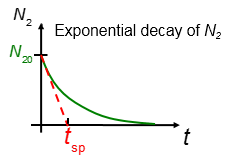
\includegraphics[scale=0.75]{ch2/image12.png}
	\captionof{figure}{ }
	\end{wrapfigure}
	La variation de la densité d'atome dans le niveau excité s'écrit
	\begin{equation}
	\frac{{{\rm{d}}{N_2}}}{{{\rm{d}}t}} =  - {A_{21}}{N_2}
	\end{equation}
	Ce qui correspond à un photon émis pour un atome désexciter. Après résolution
	\begin{equation}
	{N_2}(t) = {N_{20}}{e^{ - {A_{21}}t}}
	\end{equation}
	On parle alors de \textit{temps de vie radiatif} (temps de vie avant une émission spontanée)
	\begin{equation}
	t_{sp} = 1/A_{21}
	\end{equation}
	Il s'agit de l'inverse de $A_{21}$ et cela correspond au temps de vie de notre atome dans 
	l'état d'énergie supérieure. Ceci n'est valable que pour deux niveaux, mais on peut 
	généraliser à plusieurs niveaux
	\begin{equation}
	\frac{{{\rm{d}}{N_2}}}{{{\rm{d}}t}} =  - \sum\nolimits_k {{A_{2k}}} {N_2} =  - {N_2}/{t_{sp}}
	\end{equation}
	
	\subsection{Gain optique et forme de raie}
	Jusqu'ici nous avions considéré que les niveaux d'énergies sont bien déterminés : $\hbar
	\omega_a = E_2-E_1$ ce qui correspond à un delta de Dirac en fréquence. Ceci signifierait une 
	onde continue temporellement ce qui n'est pas possible
	\begin{center}
	Temps de vie spontané $t_{sp}\neq \infty\qquad\Rightarrow\qquad$ spectre d'émission $\neq 
	\delta(\omega-\omega_a)$
	\end{center}
	En conclusion, l'atome interagit avec un continuum de fréquences de radiation centrée 
	sur la fréquence atomique $\nu_a$ et la probabilité de transition dépend de la fréquence. On 
	définit la \textbf{forme de raie normalisée} $g(\omega)$ tel que
	\begin{equation}
	\int g(\omega)\ \text{d}\omega = 1
	\end{equation}
		
	\begin{itemize}
	\item[$\bullet$] Le taux d'absorption par unité de volume dans l'intervalle de fréquence 
	angulaire $[\omega,\omega+\delta\omega$ vaut
	\begin{equation}
	{\Gamma _{12}}(\omega )\delta \omega  = {B_{12}}{N_1}g(\omega )u(\omega )\delta \omega 
	\end{equation}
	On en tire le taux d'absorption total
	\begin{equation}
	{\Gamma _{12}} = \int {{B_{12}}u(\omega )g(\omega ){N_1}{\rm{d}}\omega } 
	\end{equation}
	\item[$\bullet$] Taux d'émission stimulée total
	\begin{equation}
	{\Gamma _{21}} = \int {{B_{21}}u(\omega )g(\omega ){N_2}{\rm{d}}\omega } 
	\end{equation}
	\end{itemize}
	A la fréquence $\omega$, le système réagit avec une certaine intensité pondérée 
	par $g(\omega)$.
	\begin{center}
	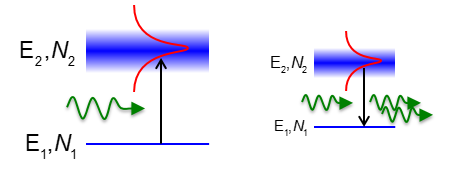
\includegraphics[scale=0.65]{ch2/image13.png}
	\captionof{figure}{Absorption à $\omega_a$ à l'énergie $E_2$ (gauche) et émission 
	stimulée (droite)}
	\end{center}
	

	\begin{wrapfigure}[7]{l}{4.5cm}
	\vspace{-5mm}
	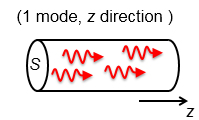
\includegraphics[scale=0.75]{ch2/image14.png}
	\captionof{figure}{ }
	\end{wrapfigure}
	Penchons-nous sur l'absorption d'une onde monochromatique à $\omega_0$. La densité 
	spectrale d'énergie s'obtient facilement : proportionnel à un delta de Dirac centré
	en $\omega_0$, à l'énergie des photons et à la densité de photon
	\begin{equation}
	u(\omega ) = \hbar {\omega _0}{n_p}\delta (\omega  - {\omega _0})
	\end{equation}
	Sachant que $\DS {B_{21}} = {B_{12}} = B = \frac{{{\pi ^2}{c^3}}}{{\hbar {\omega _0}^3{\eta ^3}}}
	{A_{21}}$, avec les deux relations intégrales que nous venons d'obtenir, on trouve
	\begin{equation}
	{\Gamma _{12}} = B\hbar {\omega _0}{n_p}g({\omega _0}){N_1},\qquad\qquad 
	{\Gamma _{21}} = B\hbar {\omega _0}{n_p}g({\omega _0}){N_2}
	\end{equation}
	Considérons le taux de variation de la densité de photon $n_p$ : celle-ci peut augmenter 
	(absorption) ou diminuer (émission spontanée et stimulée)
	\begin{equation}
	\frac{{{\rm{d}}{n_p}}}{{{\rm{d}}t}} = ({\Gamma _{21}} - {\Gamma _{12}}) + \underbrace{\text{spontaneous emission}}_{\approx 0}
	\end{equation}
	La contribution de l'émission spontanée peut être négligée : elle se produit dans toutes les 
	directions et dans toutes les fréquences, peu de chance de jouer un rôle dans l'émission laser. 
	Après ré-écriture
	\begin{equation}
	\frac{{{\rm{d}}{n_p}}}{{{\rm{d}}t}} = B\hbar {\omega _0}{n_p}g({\omega _0})({N_2} - {N_1})
	\end{equation}
	
	\begin{wrapfigure}[6]{r}{4.5cm}
	\vspace{-5mm}
	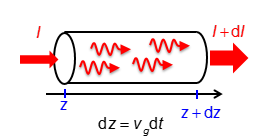
\includegraphics[scale=0.75]{ch2/image15.png}
	\captionof{figure}{ }
	\end{wrapfigure}
	En laboratoire, nous avons accès à l'intensité ($I = <S_z> (W.m^{-2})$). Sachant que 
	$I$ est le flux de photon (flux*énergie photon) et $\mathcal{J}$ est le courant (densité 
	de photon * vitesse de groupe) :
	\begin{equation}
	\left.\begin{array}{ll}
	I &= {\cal J}\hbar {\omega _0}\\
	{\cal J} &= {n_p}{v_g}
	\end{array}\right\}\quad\Rightarrow\quad I = \hbar {\omega _0}{n_p}{v_g}
	\end{equation}
	La variation de l'intensité en fonction de la position dans la cavité s'exprime alors
	\begin{equation}
	\frac{{{\rm{d}}I}}{{{\rm{d}}z}} = \hbar {\omega _0}{v_g}\frac{{{\rm{d}}{n_p}}}{{{\rm{d}}z}} = \hbar {\omega _0}\frac{{{\rm{d}}{n_p}}}{{{\rm{d}}t}}
	 = \hbar {\omega _0}B\hbar {\omega _0}g({\omega _0})({N_2} - {N_1})\frac{I}{{\hbar {\omega _0}{v_g}}} =  - \alpha I
	\end{equation}
	où $\frac{I}{{\hbar {\omega _0}{v_g}}}=n_p$. Il s'agit d'une simple relation constante*intensité : 
	cela donne lieu à une exponentielle décroissante de l'intensité lors de la propagation dans un 
	milieu. Dès lors, $\alpha$ est proportionnel au coefficient d'Einstein (échange matière-lumière) 
	mais aussi à la différence $N_1-N_2$
	\begin{equation}
	\alpha  = \frac{{\hbar {\omega _0}B{n_g}}}{c}g({\omega _0})({N_1} - {N_2}) =  - {\cal G}
	\end{equation}
	Dans un laser, on cherche à obtenir $N_2>N_1$ de façon à avoir $\mathcal{G}$ positif, soit un 
	milieu à gain.\\
	
	La seule chose qui peut changer est le $N_1-N_2$ (densité atomique en $m^{-3}$. On introduit 
	alors la section efficace $\sigma$ ($m^2$)
	\begin{equation}
	\alpha  = \frac{{{\pi ^2}{c^2}{n_g}}}{{{\eta ^3}{t_{{\rm{sp}}}}\omega _0^2}}g({\omega _0})({N_1} - {N_2}) =  - {\cal G} = \sigma ({\omega _0})({N_1} - {N_2})
	\end{equation}
	\begin{itemize}
	\item[$\bullet$] A l'équilibre thermique
	\begin{equation}
	{N_2}/{N_1} = \exp ( - \hbar {\omega _a}/{k_B}T) \ll 1\qquad\Rightarrow\qquad N_1>N_2\quad 
	\rightarrow\quad \alpha>0 : \text{ atténuation}
	\end{equation}
	\item[$\bullet$] Lors d'une \textit{inversion de la population}, loin de l'équilibre
	\begin{equation}
	{N_2} > {N_1} \Rightarrow {\cal G} > 0\ :\ \text{ amplification}
	\end{equation}
	\end{itemize}
	
	\begin{center}
		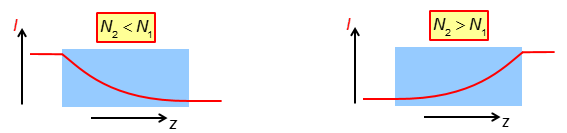
\includegraphics[scale=0.75]{ch2/image16.png}
	\captionof{figure}{Commentaires intéressants slide 30}
	\end{center}
	
	\subsection{Fonction forme de raie et mécanismes d'élargissement}
	Le but de cette sous-section est d'établir une expression de $g(\omega)$ à partir des 
	calculs des spectres d'émission et d'absorptions.
	
	\subsubsection{Largeur naturelle}
	Il s'agit du cas le plus simple, celui où l'atome se désexcite en émettant une radiation 
	à $\omega_a$. Plusieurs hypothèses sont faites 
	\begin{enumerate}
	\item Système à deux niveaux, le retour vers l'état fondamental n'est possible que par 
	émission radiative
	\item Le temps d'excitation des atomes est petite par rapport à $t_{sp}$ $\Rightarrow {N_2}(t = 0) 
	= {N_{20}}{\rm{  et   }}{N_2}(t < 0) \approx 0$
	\item Faible excitation : $1\ll R$ (émission spontanée prédominante)
	\end{enumerate}
	
	\newpage
		\begin{wrapfigure}[9]{r}{6.5cm}
	\vspace{-5mm}
	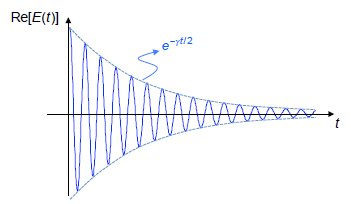
\includegraphics[scale=0.75]{ch2/image17.png}
	\captionof{figure}{ }
	\end{wrapfigure}
	L'énergie émise au cours du temps varie car la densité fait de même : l'énergie émise par 
	unité de temps par unité de volume $W$ s'exprime\footnote{Seulement un photon émis par chaque
	atome.}
	\begin{equation}
	W(t) =  - \hbar {\omega _a}\frac{{d{N_2}}}{{dt}} = \frac{{\hbar {\omega _a}}}{{{t_{{\rm{sp}}}}}}{N_{20}}\exp ( - t/{t_{{\rm{sp}}}}){\rm{ }}(t \ge 0)
	\end{equation}
	Le champ EM classique associé à cette désexcitation est un champ oscillant à $\omega_a$ et dont 
	l'amplitude décroit au cours du temps.\\

	Calculons l'amplitude spectrale (transformée de Fourier, le tilde désigne le domaine des 
	fréquences)
	\begin{equation}
	\tilde E(\omega ) = \int\limits_{ - \infty }^{ + \infty } {E(t)} \,{\rm{exp(}}i\omega t{\rm{)d}}t = \int\limits_0^{ + \infty } {{E_0}{\rm{exp(}} - t/2{t_{sp}} - i{\omega _a}t{\rm{)}}\,} {\rm{exp(}}i\omega t{\rm{)}}\,{\rm{d}}t{\rm{  }}  = \int\limits_0^{ + \infty } {{E_0}\exp \left\{ {t[i(\omega  - {\omega _a}) - 1/2{t_{sp}}]} \right\}{\rm{d}}t}
	\end{equation}
	Après intégration
	\begin{equation}
	\tilde E(\omega ) = \frac{{{E_0}}}{{ - i(\omega  - {\omega _a}) + 1/2{t_{sp}}}}
	\end{equation}
	Le spectre vaut alors
	\begin{equation}
	\tilde {\cal I}(\omega ) = |\tilde E(\omega ){|^2}\quad\Rightarrow\quad 
	\tilde {\cal I}(\omega ) = \frac{{E_0^2}}{{{{(\omega  - {\omega _a})}^2} + {\gamma ^2}/4}}
	\end{equation}
	Ceci n'est rien d'autre qu'une lorentzienne avec un profil d'épaisseur $\gamma = 1/t_{sp}=A_{21}$ 
	(spectre d'émission). Si l'atome reste très peu longtemps dans son état excité $g(\omega)$ sera 
	important mais s'il reste très longtemps dans le niveau excité $g(\omega)$ sera très 
	petit\footnote{Calcul de la normalisation slide 33 passé}
	\begin{equation}
	g(\omega ) = \frac{K}{{1 + {{(\frac{{\omega  - {\omega _a}}}{{\gamma /2}})}^2}}}
	\end{equation}
	où $K=\frac{2}{\pi\gamma}, \gamma=1/t_{sp}$ (largeur spectrale (largeur totale à la moitié 
	du maximum) : $\Delta\omega = \gamma$.
	
	Jusqu'ici nous n'avons travailler qu'à deux niveaux : il est possible de généraliser l'expression 
	de $\gamma$ (forme de raie) avec le principe d'incertitude temps-énergie : il suffit de considérer 
	plusieurs coefficients d'Einstein, un pour chaque transition possible
	\begin{enumerate}
	\item Pour le niveau supérieur : $\Delta {{\rm{E}}_s} = \hbar \Delta {t_s}^{ - 1} = \hbar \sum
	\nolimits_k {{A_{sk}}} $
	\item Pour le niveau inférieur : $\Delta {{\rm{E}}_i} = \hbar \Delta {t_i}^{ - 1} = \hbar \sum\nolimits_l {{A_{\;il}}} $
	\end{enumerate}

	\begin{wrapfigure}[7]{l}{3.5cm}
	\vspace{-5mm}
	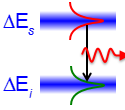
\includegraphics[scale=0.85]{ch2/image18.png}
	\captionof{figure}{ }
	\end{wrapfigure}
	En effet, le système ne reste qu'un certain temps sur les niveaux excités : il y a une incertitude
	 sur les niveaux d'énergie et donc une incertitude sur les photons émis, c'est ce que traduit
	 $g(\omega)$. La largeur de raie naturelle tient compte de ceci
	 \begin{equation}
	{\gamma _n} = \Delta \omega  = \frac{{\Delta {{\rm{E}}_s} + \Delta {{\rm{E}}_i}}}{\hbar } = {\gamma _s} + {\gamma _i} = \sum\limits_{l\,\,t.q.\hfill\atop
\scriptstyle{{\rm{E}}_k} < {{\rm{E}}_s}\hfill} {{A_{\;sk}}}  + \sum\limits_{l\,\,t.q.\hfill\atop
\scriptstyle{{\rm{E}}_l} < {{\rm{E}}_i}\hfill} {{A_{\;il}}} 
	 \end{equation}
	 
	 \subsubsection{Mécanisme d'élargissement homogène}
	 Il existe des principes physiques qui vont "agrandir" la grandeur naturelle (qui est la plus 
	 petite que possible). Il en existe deux type (selon le type de laser)
	 \begin{enumerate}
	 \item Homogène : tous les atomes sont impactés de la même façon par ce mécanisme, ils subissent 
	 tous le même "élargissement".
	 \item Inhomogène : le milieu atomique est divisé en classe d'atomes qui interagissent tous 
	 un peu différemment.
	 \end{enumerate}
	 Voyons ici différent mécanismes homogènes.\\
	 
	 \textsc{Transition non-radiative}\\
	 Celles-ci sont dues à des collisions entre les atomes (laser à gas comme dans le laser
	 He-Ne) où les interactions avec des photons (laser solide)\footnote{Nous avions vu l'incertitude 
	 temps-énergie: plus un atome reste longtemps dans un état, plus cet état est incertain.}
	 \begin{center}
 	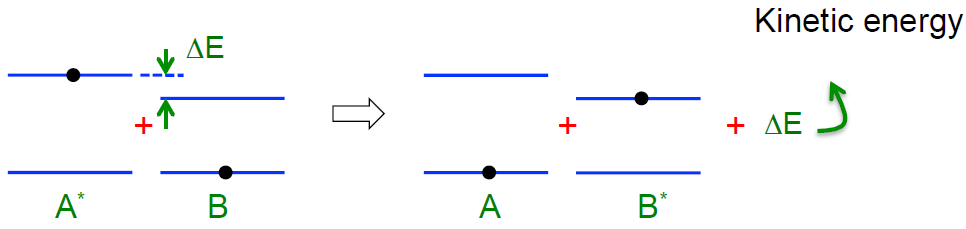
\includegraphics[scale=0.5]{ch2/image19.png}
	\captionof{figure}{La différence entre les deux niveaux part en énergie cinétique}
	 \end{center}
	 \begin{equation}
	\gamma  = {\gamma _n} + 1/{t_{{\rm{nr - low}}}} + 1/{t_{{\rm{nr - up}}}}
	 \end{equation}
	 avec $t_{nr-low/up}$ le temps de vie non radiatif de l'état haut/bas.\\
	 
	 \textsc{Collisions (sans transitions)}\\
	 Cet effet est plus subtil : il se déroule entre les atomes pour les gaz et avec les 
	 phonons pour les solides (pas de modification du temps de vie). Considérons un atome
	 oscillant. Si un second atome arrive dans son environnement avec son propre champ électrique, 
	 il va modifier les écarts d'énergie entre les niveaux : effet Stark. Ceci se traduit par un 
	 déphasage durant l'émission radiative, qui est aléatoire. 
	 
	 	 \begin{center}
 	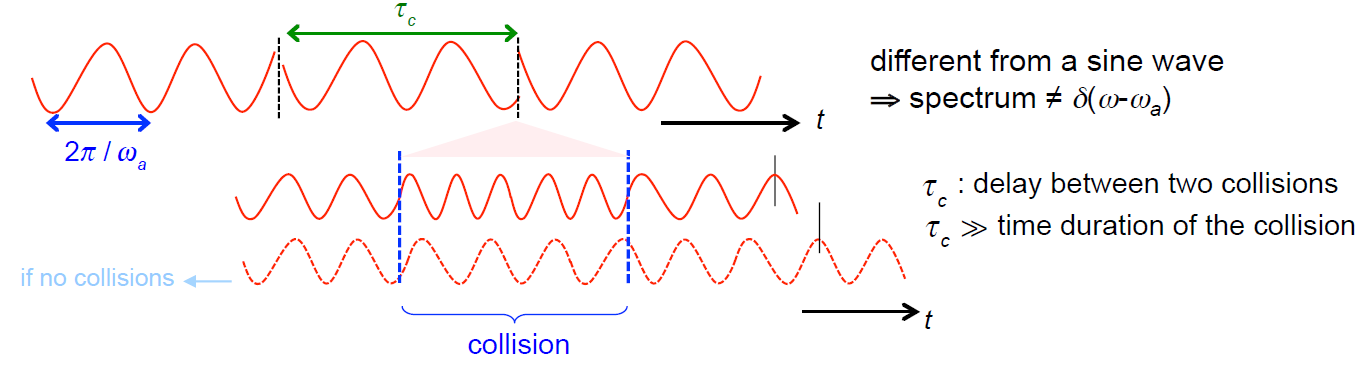
\includegraphics[scale=0.45]{ch2/image20.png}
	\captionof{figure}{ }
	 \end{center}
	 
	 La solution est entrecoupée de sauts de phase : $\tau_c$ est l'intervalle entre deux collisions 
	 qui est supposé beaucoup plus grand que le temps de la collision. 
	 Si l'on a une onde continue le spectre n'est qu'un Delta de Dirac mais comme la solution est 
	 entrecoupée de sauts de phase, le spectre se voit élargi.\\
	 
	 Durant l'intervalle $\tau_c$, le dipôle atomique oscille à $\omega_a$, le champ est donc 
	 une exponentielle proportionnelle à ce temps
	 \begin{equation}
	 E(t) \propto\exp(-i\omega_at')\qquad t<t'<t+\tau
	 \end{equation}
	 Le spectre correspondant vaut
	 \begin{equation}
	 \tilde E(\omega ;{\tau _c}) \propto \int\limits_t^{t + {\tau _c}} {{{\rm{e}}^{ - i{\omega _a}t'}}} {{\rm{e}}^{i\omega t'}}{\rm{d}}t' = \frac{{{\rm{exp(}}i\Delta \omega {\tau _c}{\rm{)}} - 1}}{{i\Delta \omega }}{{\rm{e}}^{i\Delta \omega t}}{\rm{ }}
	 \end{equation}
	 où $\Delta\omega = \omega-\omega_a$. L'intensité spectrale est donnée par le module carré de 
	 cette transformée de Fourier
	 \begin{equation}
	 \tilde I(\omega ;{\tau _c}) \propto \frac{{{{(\cos [\Delta \omega {\tau _c}] - 1)}^2} + {{\sin }^2}[\Delta \omega {\tau _c}]}}{{\Delta {\omega ^2}}}{\rm{  = }}\frac{{2 - 2\cos [\Delta \omega {\tau _c}]}}{{\Delta {\omega ^2}}}
	 \end{equation}
	 Nous allons sommer sur tous les spectres en tenant compte du poids de chaque spectre : 
	 probabilité. On suppose que le saut de phase est aléatoire et que $p(\tau_c)$ est la 
	 probabilité que le temps entre deux collisions soit $\tau_c$ :
	 \begin{equation}
	  \tilde I(\omega ) \propto \int\limits_0^\infty  {\tilde I(\omega ;{\tau _c})p({\tau _c}){\rm{d}}{\tau _c}}
	 \end{equation}
	 La théorie cinétique nous donne une expression de la distribution de probabilité du délai entre
	 deux collisions 
	 \begin{equation}
	 p({\tau _c}){\rm{d}}{\tau _c} = 1/{\tau _0}\exp ( - {\tau _c}/{\tau _0}){\rm{d}}{\tau _c}
	 \end{equation}
	 Pour calculer l'intensité, on s'intéresse à la valeur moyenne de ce délai entre deux collisions
	 \begin{equation}
	 \int\limits_0^\infty  {{\tau _c}p({\tau _c}){\rm{d}}{\tau _c}}  = {\tau _0}
	 \end{equation}
	 Il ne reste plus qu'à calculer
	 \begin{equation}
	 \tilde I(\omega ) \propto \int\limits_0^\infty  {\frac{{1 - \cos [\Delta \omega {\tau _c}]}}{{\Delta {\omega ^2}}}{{\rm{e}}^{ - {\tau _c}/{\tau _0}}}{\rm{d}}{\tau _c}} 
	 = \frac{1}{{2\Delta {\omega ^2}}}\int\limits_0^\infty  {(2{{\rm{e}}^{ - {\tau _c}/{\tau _0}}} - {{\rm{e}}^{ - (1/{\tau _0} - i\Delta \omega ){\tau _c}}} - {{\rm{e}}^{ - (1/{\tau _0} + i\Delta \omega ){\tau _c}}}){\rm{d}}{\tau _c}}
	 \end{equation}
	 Après intégration
	 \begin{equation}
	 \tilde I(\omega ) \propto \frac{1}{{2\Delta {\omega ^2}}}\left[ {2{\tau _0} - \frac{1}{{1/{\tau _0} - i\Delta \omega }} - \frac{1}{{1/{\tau _0} + i\Delta \omega }}} \right] = \frac{{{\tau _0}}}{{{{(1/{\tau _0})}^2} + \Delta {\omega ^2}}}
	 \end{equation}
	 Il s'agit d'une lorentzienne ! En normalisant à l'unité, on peut trouver la forme de 
	 raie $g(\omega)$\footnote{Si on considère que la forme de raie est rectangulaire (vrai 
	 si très petit) : $\int g(\omega)d\omega = 1\Leftrightarrow g(\omega) = 1/\Delta\omega$.}
	 \begin{equation}
	 g(\omega ) = \frac{{{\tau _0}}}{\pi }\frac{1}{{1 + \Delta {\omega ^2}/{{({\gamma _{{\rm{co}}}}/2)}^2}}}
	 \end{equation}
	 C'est également un profil lorentzien de largeur $\gamma_{co} = 2/\tau_0$.
	 
	 \newpage
	 	\begin{wrapfigure}[12]{l}{5.5cm}
	\vspace{-3mm}
	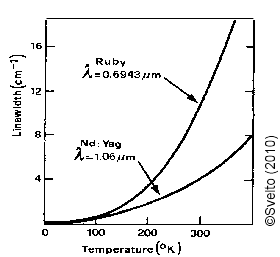
\includegraphics[scale=0.65]{ch2/image21.png}
	\captionof{figure}{ }
	\end{wrapfigure}
	 On peut comptabiliser la largeur naturelle avec la modification obtenue par les collisions : 
	 décroissance exponentielle de l'amplitude d'oscillation et saut de phases aléatoires
	 \begin{equation}
	 {\gamma _{\rm{h}}} = {\gamma _{\rm{n}}} + 1/{t_{nr}} + 2/{\tau _0}
	 \end{equation}
	 En pratique, on remarque que le spectre d'émission est beaucoup plus large que ce à quoi 
	 on s'attend pour la décroissance exponentielle : ceci est du à l'influence de la température. 
	 Quand celle-ci augmente, la densité de photon augmente et le temps entre deux collisions diminue,
	 causant un élargissement de la largeur spectrale.
	 
	 \subsubsection{Élargissement inhomogène}
	 Il s'agit d'un mécanisme qui fait que ça ne se déroule pas toujours de la même façon au 
	 niveau des interactions lumière-matière. Le milieu est donc un ensemble de groupe d'atomes
	 ayant une fréquence de résonance différente. Il faut donc connaître la distribution statistique
	 des groupes d'atomes ayant une fréquence $\omega_c$
	 \begin{equation}
	 F(\omega_c) : \text{fonction de distribution statistique normalisée à l'unité}
	 \end{equation}
	 On a donc que $\delta N_c = F(\omega_c)N\delta\omega_c$ est le nombre d'atomes entrant en 
	 résonance pour un champ électromagnétique de fréquence dans $[\omega_c,\omega_c+\delta
	 \omega_c]$.\\
	 
	 Chaque groupe d'atome $\delta N_c$ interagit avec une onde optique de fréquence $\omega$ 
	 proportionnelle à $g_h(\omega-\omega_c)$ où $g_h$ est la forme de raie normalisée centrée 
	 en $\omega=0$. La contribution de chaque groupe d'atome au taux d'émission stimulée à la 
	 fréquence $\omega$ vaut donc
	 \begin{equation}
	 {\Gamma _{21,c}} = {B_{21}}u(\omega ){g_h}({\omega _c} - \omega )\delta {N_{2,c}}
	 \end{equation}
	 On retrouve le coefficient d'Einstein, la densité spectrale d'énergie et $g$ qui permet de 
	 ne considérer que la fraction correspondante à la fréquence qui nous intéresse. Pour obtenir 
	 le taux d'émission stimulée total, il faut intégrer
	 \begin{equation}
	 \Gamma  = \sum\nolimits_c {{\Gamma _{21,c}}}  = {B_{21}}u{N_2}\underbrace{\int_0^\infty  {{g_h}({\omega _c} - \omega )F({\omega _c})d{\omega _c}} }_{g = F*g_h}
	 \end{equation}
	 La nouvelle forme de raie est donnée par la convolution entre l'élargissement homogène et
	 la fonction de distribution $F$. Cette forme tient ainsi compte des élargissements 
	 non-homogène. Dès lors, pour que l'élargissement inhomogène affecte le fonctionnement du 
	 laser, il faut que $F$ soit au moins aussi large que $g_h$.\\


	 Passons en revue deux exemples d'élargissement non-homogène
	 \begin{enumerate}
	 \item Doppler. Affecte tous les lasers à gaz : on peut créer des sous-ensemble d'atomes qui 
	 réagissent à des fréquences différentes. Si les photons vont vers la droite et l'atome également, 
	 la fréquence sera plus importante et inversement. La vitesse $c$ devient alors une certaine 
	 vitesse $v(z)$ à cause de ce décalage
	 \begin{equation}
	 \omega\to \omega-\vec{k}.\vec{v} = \omega-(\pm k.v_z)
	 \end{equation}
\begin{center}
	 	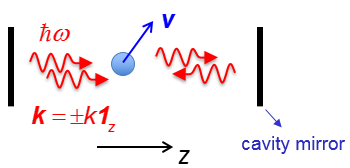
\includegraphics[scale=0.65]{ch2/image22.png}
	\captionof{figure}{ }
\end{center}
	 Pour des atomes de masse $m$ à température $T$, la distribution des vitesses est celle de Maxwell
\begin{equation}
f({v_z}) = {\left( {\frac{m}{{2\pi {k_B}T}}} \right)^{1/2}}\exp ( - \frac{{mv_z^2}}{{2{k_B}T}})
\end{equation}
Exprimée en fréquence
\begin{equation}
F(\omega ) = {\left( {\frac{m}{{2\pi {k_B}T{k^2}}}} \right)^{1/2}}\exp ( - \frac{m}{{2{k_B}T}}\frac{{{{(\omega  - {\omega _a})}^2}}}{{{k^2}}})
\end{equation}
Le profil tenant compte de l'élargissement homogène et inhomogène est donné par la convolution 
entre une lorentzienne et une gaussienne.
\begin{equation}
g(\omega ) = \int {{g_h}({\omega _c} - \omega )} F({\omega _c}){\rm{d}}{\omega _c}
\end{equation}
Il s'agit d'un \textit{intégrale de Voigt}. Si $\gamma_h\ll k\sqrt{2k_BT/m}$ alors
\begin{equation}
g(\omega ) \approx \frac{{{{\mathop{\rm e}\nolimits} ^{ - \frac{{{{[\omega  - {\omega _a}]}^2}}}{{{k^2}2{k_B}T/m}}}}}}{{k\sqrt {2\pi {k_B}T/m} }}\qquad \Rightarrow\qquad \Delta \omega  \approx 1.66k\sqrt {2{k_B}T/m} 
\end{equation}
\begin{center}
	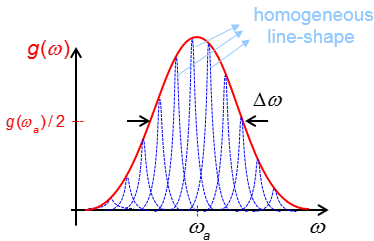
\includegraphics[scale=0.65]{ch2/image23.png}
	\captionof{figure}{ }
\end{center}
\item Environnement. Les environnements amorphes comme le verre : les distances entre chaque atomes 
ne sont pas connues. Si l'environnement électrique est différent il y aura un 
déplacement des niveaux d'énergies différent (Stark), \dots Si le milieu est plus ordonnée par 
exemple YAG (cristallin) à la place de Nd glass (amorphe) l'élargissement est moins important.
	 \end{enumerate}
	 
	 
	 
	 
	 
	 
	 
	 
	 
	 
	 
	 
	 
	 
	 
	 
	 
	 
	 
	 
	 
	 
	 